%%%%%%%%%%%%%%%%%%%%%%%%%%%%%%%%%%%%%%%%%%%%%%%%%%%%%%%%%%%%%%%%%%%%%%%%%%%%%%%%
%                                                                              %
%   File:     metholodgy.tex                                               %
%   Document: XXX	                                                       %
%   Author:   Freismuth David                                              %
%	Date:	  22.JUN.2018                                                  %
%   Content:  Contains the Metholodgy section of the Bachelor thesis.      %
%                                                                              %
%%%%%%%%%%%%%%%%%%%%%%%%%%%%%%%%%%%%%%%%%%%%%%%%%%%%%%%%%%%%%%%%%%%%%%%%%%%%%%%%

%%%%%%%%%%%%%%%%%%%%%%%%%%%%%%%%%%%%%%%%%%%%%%%%%%%%%%%%%%%%%%%%%%%%%%%%%%%%%%%%
\section{Metholodgy}

We use Scrapy, a Python web scraping library, to 
automatically obtain design files and corresponding meta-information for each 
design that is published via \gls{oc}. We are interested in the following data:

\begin{enumerate}

	\item{\gls{url} to the compressed design archive}

	\item{The name of the design project}

	\item{The \gls{hdl} in which the design is specified and implemented}

	\item{The category in which a design is listed on \gls{oc}}
	
	\item{The \gls{hdl} files of the design}
	
\end{enumerate}

\subsection{Learn Process}

\subsubsection{Scraping OpenCores project web sites} 
The scraped data is temporarily stored into Python class objects. The information 
in these objects are written to a .JSON file, in order to make them persistent (such
that we do not have to scrape the entire \gls{oc} web site every time we use our 
classification framework). For this .JSON file, a specific format has been defined, 
so information can be imported from other sources then scrapy aswell. 

\begin{figure}[tb]
	\centering
	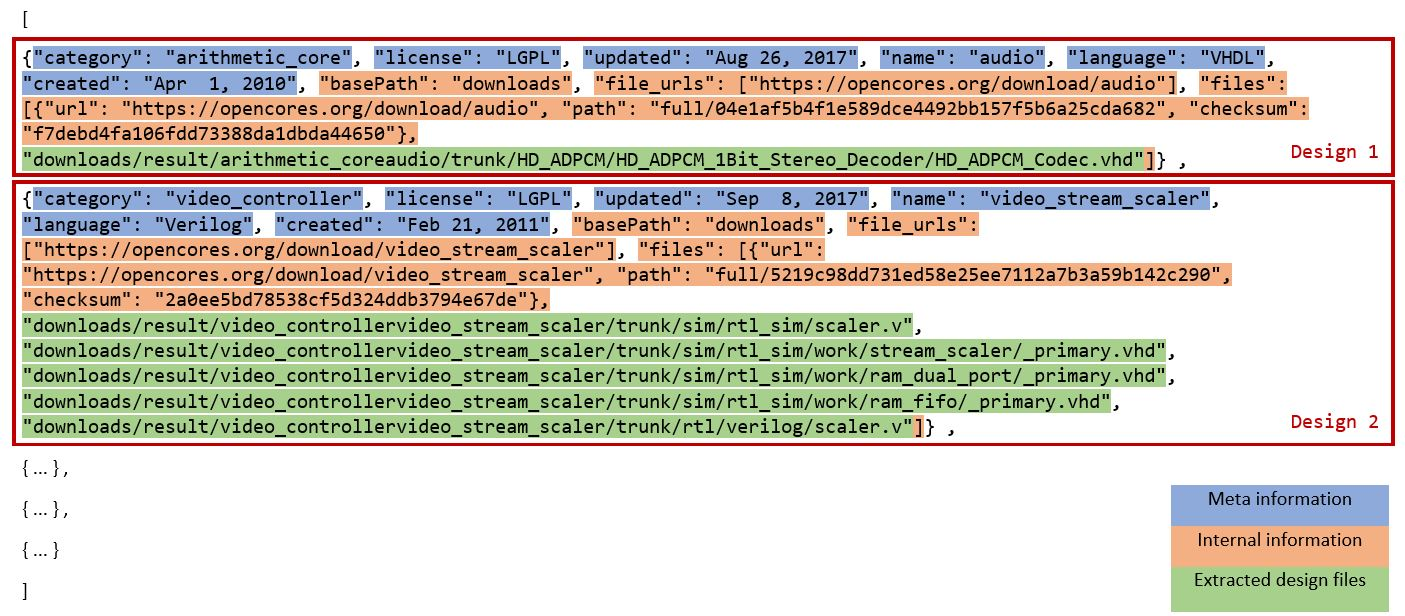
\includegraphics[width=\textwidth,keepaspectratio]{../pictures/jsonFileFormatDescription.JPG}
	\caption{.JSON File Format Description}
	\label{fig:jsonFormat}
\end{figure}

Figure \Cref{fig:jsonFormat} shows an example of the content of the .JSON file. 

\subsubsection{Downloading OpenCores projects}
The Scrapy python module provides the functionallity to automatically download and
store files that are associated with a Hardware design project, to a predefined
folder. Since \gls{oc} requires an account to be able to download hardware designs, 
we use a scrapy internal function to send a POST request to the \gls{oc} webpage,
in order to authorize ourselfs. 

Because all project files from the \gls{oc} database are provided as tar.gz archives,
we introduced an additional decompression step.  

\subsubsection{Decompressing design files} 
Projects from \gls{oc} are solely provided as *.tar.gz compressed archive. The \gls{python}
module tarfile enables the extraction of those archives. Additionally 
to the decompression, we sort the project files into folders corresponding to 
their associated hardware category (as stated by \gls{oc}). After that, the file 
endings of the files are analysed. If those endings indicate a \gls{hdl} file, the path 
to this file is added to the aforementioned .JSON file, in order to be able to
address the design files of a project in later steps.

\subsubsection{Reading designs into synthesis tool} 
After the design has been decompressed, it is time to let the synthesis tool 
yosys read the design files and synthesise them into a text file format. In 
order to do this, yosys expects a yosys script file, which holds all yosys commands 
that should be executed on a set of files. This script file can either be provided
by the user before a programm run, or a generic one can be generated automatically 
during a programm run, according to the files that have been provided with the 
.JSON file. 

The synthesis tool's frontend is chosen based on the language of each design file.
For \gls{vhdl} and SystemVerilog, the \lstinline{verific} frontend is used. For Verilog,
we use the \lstinline{read_verilog} frontend. Once any combination of \gls{hdl} files
has been loaded, a synthesize run attempts to generate a single HDL file from the provided
files, which solely contains primitive logic blocks. 

Since yosys does not support automatic dependency recognition of vhdl files, a custom solution
had to be found, to determine the load order of vhdl files (in the case that the user decides
that yosys scripts should be generated automatically). To accomplish this, we slightly modified 
the Vunit python project, which offers a function to return the \gls{vhdl} 
files in an ordered list. The vhdl files can then be loaded in the order dictated by this list.  

\subsubsection{Naming designs} 
Each design that is read by the synthesis tool is named after the project from
which the design files are downloaded. From then, the design name is the main
reference for each design and serves as identification feature in all
subsequent steps.

\subsubsection{Matching designs against standard pattern vector}
\subsubsection{Calculating clusters of design match vectors}

\subsection{Verification}



